\subsubsection{Project}
	In the UPRM system, projects will refer to any new paper or report that the researcher(s) will be involved in. The user has to be able to create multiple projects and keep track of progress by means of a timeline and project specific sub-deadlines.
	The access rights and privileges to each operation will have to be checked before any operation is executed.\\
	
	\centerline{\fbox{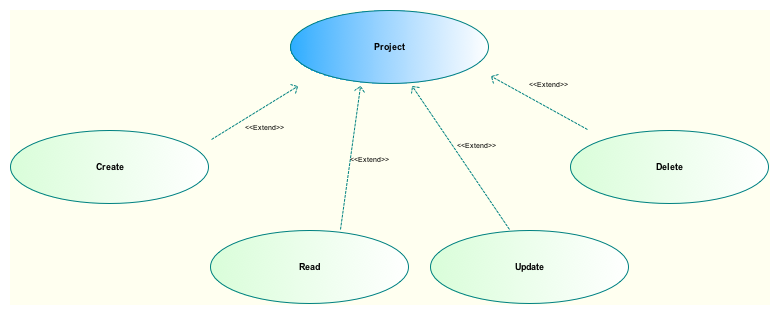
\includegraphics[width=\linewidth]{CRUD/uprm_CRUD_Overview.png}}}
	
	\setcounter{secnumdepth}{4}
	\paragraph{Create Project\\}
	Once a user has been successfully authenticated by the UPRM system, the user should be able to create a new project. On creation of a new project, the user will have to provide the following details:
	\begin{itemize}
		\item Name(or Title) of the new project.
		\item A short description of the new project.
		\item An overall project deadline.
		\item Optional project specific sub-deadlines to track progress. The default timeline will be from project creation date to overall project deadline and a 1\% progress.
	\end{itemize} 
	
	\setcounter{secnumdepth}{5}
	\subparagraph{Use Case\\}
		Use case for the creation of projects:\\
		\centerline{\fbox{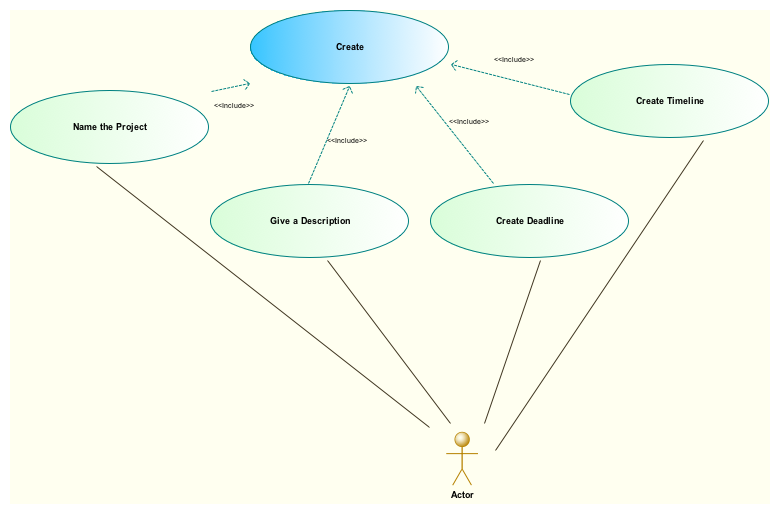
\includegraphics[width=\linewidth]{CRUD/uprm_create.png}}}
	
	\subparagraph{Classes and Objects\\}
	test
	